\graphicspath{{./figures/capitolo8/}}
\lstset{inputpath = ./programs/capitolo8}
\pgfplotstableset{search path = ./tables/capitolo8}

\chapter{Metodi Runge-Kutta}

In quest'ultimo capitolo torneremo ad occuparci di metodi numerici
per la discretizzazione del problema di Cauchy
\begin{equation} \label{eq:problema-di-cauchy-cap8}
\left\{
\begin{aligned}
y'(t)  &= f(t,y(t)) \quad \text{per ogni $t \in [t_0,T]$}, \\
y(t_0) &= y_0 \in \R^m,
\end{aligned}
\right.
\end{equation}
e vedremo come, attraverso l'introduzione di metodi numerici più flessibili,
sarà possibile superare la seconda barriera di Dahlquist e allo stesso
tempo trattare in modo qualitativamente corretto non solo problemi dissipativi,
ma anche problemi conservativi di tipo hamiltoniano (si parla in questo caso
di integratori geometrici). Nel Capitolo 3, l'idea alla base dei metodi numerici
multistep era quella di discretizzare direttamente l'equazione differenziale
\eqref{eq:problema-di-cauchy-cap8} tramite un'opportuna equazione alle differenze;
in questo capitolo vedremo invece un approccio basato sulla forma integrale
dell'equazione \eqref{eq:problema-di-cauchy-cap8}. Sia
$t_0 < t_1 < \dots t_N = T$ una partizione dell'intervallo $[t_0,T]$,
non per forza uniforme. Allora, a ogni passo temporale discreto
possiamo scrivere che
\[
y(t_{n+1}) = y(t_n) + \int_{t_n}^{t_{n+1}} f(t,y(t)) \dt.
\]
Come nel Capitolo 3, indichiamo con $y_n$ l'approssimazione di $y(t_n)$
fornita dal metodo numerico e con $h$ l'incremento temporale $t_{n+1}-t_n$.
Per discretizzare l'integrale dell'equazione precedente possiamo ricorrere
a una formula di quadratura con $s$ nodi
\[
t_n + c_1 h,\, \dots,\, t_n + c_s h \qquad 0 \leq c_1 \leq \dots \leq c_s \leq 1
\]
e con pesi $b_1, \dots, b_s$:
\vspace{-1em}
\begin{equation} \label{eq:sistema-yn+1-runge-kutta}
y_{n+1} = y_n + h \sum_{i=1}^s b_i f(t_n+c_i h, y(t_n + c_i h)).
\end{equation}
Il valore $s$ è detto \emph{numero di stadi} del metodo.
A questo punto, rimane solo da decidere come approssimare i valori
$y(t_n+c_i h)$ (tali approssimazioni verranno indicate con $Y_i$).
L'idea alla base dei \emph{metodi Runge-Kutta} è quella di ricorrere
nuovamente al teorema fondamentale del calcolo
\[
y(t_n + c_i h) = y(t_n) + \int_{t_n}^{t_n+c_i h} f(t,y(t)) \dt,
\]
e di approssimare anche questi nuovi integrali con delle formule
di quadratura basate sugli stessi nodi $c_1, \dots, c_s$ e con pesi $a_{ij}$:
\begin{equation} \label{eq:sistema-Yi-runge-kutta}
Y_i = y_n + h \sum_{j=1}^s a_{ij} f(t_n + c_j h, Y_j).
\end{equation}
In questo modo, la \eqref{eq:sistema-yn+1-runge-kutta} e la
\eqref{eq:sistema-Yi-runge-kutta} formano un sistema chiuso di $s+1$ equazioni
vettoriali nelle incognite $Y_1,\dots,Y_s,y_{n+1}$, la cui soluzione
ci permette di avanzare nel tempo di una quantità $h = t_{n+1}-t_n$.
I coefficienti $a_{ij}$ formano una matrice $A$ detta \emph{matrice di Butcher},
mentre i coefficienti $b_i$ e $c_i$ formano dei vettori $b$ e $c$ detti
rispettivamente \emph{vettore dei pesi} e \emph{vettore dei nodi}.
La terna $(A,b,c)$ caratterizza in modo univoco il particolare metodo Runge-Kutta
e solitamente viene riportata sotto forma di \emph{tableau di Butcher}
\[
\renewcommand\arraystretch{1.4}
\begin{array}
{c|c}
c & A \\
\hline
 & b^{\mathrlap{\scriptscriptstyle T}} \\
\end{array}
\]
Osserviamo che, a differenza dei metodi lineari multistep, i metodi Runge-Kutta
sono metodi a un solo passo, perché $y_{n+1}$ dipende unicamente da $y_n$
e non dai valori $y_i$ precedenti.

Anche in questo contesto, ha senso distinguere tra metodi espliciti e metodi
impliciti. Se la matrice $A$ è strettamente triangolare inferiore, le
equazioni \eqref{eq:sistema-Yi-runge-kutta} possono essere risolte
al variare di $i = 1,\dots,s$ tramite delle semplici sostituzioni in avanti,
quindi la complessità computazionale di ogni passo è bassa (pari a $O(m)$)
e per questo si parla di \emph{metodo Runge-Kutta esplicito}.
Se invece $A$, pur essendo triangolare inferiore, ha elementi non nulli
sulla diagonale, allora l'equazione \eqref{eq:sistema-Yi-runge-kutta} diventa
\[
Y_i - ha_{ii}f(t_n+c_i h,Y_i)
= y_n + h \sum_{j=1}^{i-1} a_{ij} f(t_n + c_j h, Y_j)
\eqd g_n,
\]
e in questo caso si parla di \emph{metodo Runge-Kutta semi-implicito}.
Osserviamo che ogni equazione nonlineare \eqref{eq:sistema-Yi-runge-kutta}
può essere risolta separatamente, purché lo si faccia nell'ordine giusto,
e che sotto l'ipotesi $h \abs{a_{ii}} L < 1$ la soluzione $Y_i$
di ciascuna equazione esiste ed è unica per il teorema di punto fisso di Banach.
Infine, se $A$ ha elementi non nulli al di sopra della diagonale, le $s$
equazioni \eqref{eq:sistema-Yi-runge-kutta} formano necessariamente un
unico sistema nonlineare di $sm$ equazioni scalari che non può essere
a priori semplificato. Almeno la notazione, però, può essere resa più compatta:
siano $\otimes$ il prodotto di Kronecker tra matrici e $Y,f(Y),e$
i vettori colonna
\[
Y = \begin{pmatrix}
Y_1 \\ 
\vdots \\ 
Y_s \\
\end{pmatrix} \in \R^{sm}, \quad
f(Y) = \begin{pmatrix}
f(t_n+c_1 h, Y_1) \\ 
\vdots \\ 
f(t_n+c_s h, Y_s) \\
\end{pmatrix} \in \R^{sm}, \quad
e = \begin{pmatrix}
1 \\ 
\vdots \\ 
1 \\
\end{pmatrix} \in \R^{s}.
\]
Allora il sistema delle equazioni \eqref{eq:sistema-Yi-runge-kutta} corrisponde a
\[
F(Y) \deq Y - e \otimes y_n - h (A \otimes I_m) f(Y) = 0.
\]
In questo caso si parla di \emph{metodo Runge-Kutta implicito}, e si può
dimostrare che l'ipotesi giusta per applicare il teorema di punto fisso
di Banach è $h \norm{A} L < 1$.
Nella pratica computazionale, ha senso distinguere i metodi semi-impliciti
da quelli impliciti, perché c'è un vantaggio non trascurabile nel risolvere
$s$ sistemi di dimensione $m$ rispetto a un solo sistema di dimensione $sm$.

Come nel caso dei metodi lineari multistep, ci sono buoni motivi per evitare
di risolvere i sistemi non lineari mediante iterazioni di punto fisso.
La matrice jacobiana di $F(Y)$, necessaria per poter impiegare
il metodo di Newton o una delle sue varianti, è la seguente:
\[
F'(Y) = I_{sm} - h (A \otimes I_m) \begin{pmatrix}
\partial_y f(t_n+c_1 h,Y_1) & & \\
& \ddots & \\
& & \partial_y f(t_n+c_s h,Y_s) \\
\end{pmatrix}.
\]
Nel caso del metodo di Newton stazionario, l'unica jacobiana di $f$ da calcolare
a ogni passo sarà $J_0 = \partial_y f(t_n,y_n) \approx \partial_y f(t_n+c_i h, Y_i)$,
quindi l'espressione precedente può essere semplificata:
\[
F'(Y) \approx I_{sm} - h (A \otimes I_m)(I_s \otimes J_0) = I_{sm} - h (A \otimes J_0).
\]
A conclusione di questo paragrafo, riportiamo il Programma \ref{prog:runge-kutta},
che illustra una possibile implementazione di un generico metodo Runge-Kutta
in funzione dei coefficienti $(A,b,c)$. Possiamo osservare le numerose
somiglianze a livello di scelte implementative con l'analogo
Programma \ref{prog:lmf} del Capitolo 3, che illustrava un generico metodo
lineare multistep. I sistemi non lineari nel caso semi-implicito e implicito
sono risolti dai Programmi \ref{prog:RK-semiimplicit-solver} e
\ref{prog:RK-implicit-solver} utilizzando il metodo di Newton stazionario.
La funzione \code{numerical\_jacobian} è la stessa del Capitolo 3
(Programma \ref{prog:lmf-numerical-jacobian}).

\clearpage

\lstinputlisting[label=prog:runge-kutta, caption={Implementazione
di un generico metodo Runge-Kutta.}]{runge_kutta.m}

\lstinputlisting[float=p, label=prog:RK-semiimplicit-solver, caption={Metodo di Newton
stazionario per metodi Runge-Kutta semi-impliciti.}]{RK_semiimplicit_solver.m}

\lstinputlisting[float=p, label=prog:RK-implicit-solver, caption={Metodo di Newton
stazionario per metodi Runge-Kutta impliciti.}, linerange={1-6,10-31}]{RK_implicit_solver.m}

\clearpage

\section{Proprietà dei metodi Runge-Kutta}

Per quanto riguarda le proprietà dei metodi Runge-Kutta, valgono definizioni
del tutto analoghe a quelle date per i metodi lineari multistep, anche se
qui preferiamo non riportare i dettagli: si può dunque parlare di ordine
di convergenza, di errore di troncamento locale, di consistenza, di zero-stabilità
e di assoluta stabilità. %anche in questo contesto

Consideriamo il problema $y'(t) = 0$, $y(t_0) = y_0$ associato all'analisi
di zero-stabilità di un metodo numerico per equazioni differenziali ordinarie.
Dato che $f(t,y) \equiv 0$, è immediato verificare che l'equazione
\[
y_{n+1} = y_n + h \sum_{i=1}^s b_i f(t_n+c_i h, Y_i)
\]
con cui un generico metodo Runge-Kutta avanza nel tempo si semplifica in
$y_{n+1} = y_n$, quindi possiamo concludere che i metodi Runge-Kutta
sono incondizionatamente zero-stabili.
Allora, dato che anche per i metodi Runge-Kutta si può dimostrare un risultato
analogo al Teorema \ref{teor:ordine-convergenza-lmf}, cioè che consistenza
e zero-stabilità sono condizioni sufficienti per la convergenza, si ha che
la classe dei metodi Runge-Kutta convergenti coincide con quella
dei metodi Runge-Kutta consistenti.
La condizione sui coefficienti $(A,b,c)$ di un metodo Runge-Kutta che caratterizza
la consistenza è
\[
\sum_{i=1}^s b_i = 1,
\]
ma a differenza dei metodi lineari multistep non esiste una caratterizzazione
dei metodi di ordine superiore semplice come quella del Teorema \ref{teor:ordine-lmf}:
i vincoli che si ottengono dalla formula di Taylor non sono lineari, non sono
tutti indipendenti e crescono in numero molto velocemente in funzione
dell'ordine $p$.
Per questo motivo teoremi come l'\ref{teorema-ordine-convergenza-HBVM},
che vedremo a breve, svolgono un ruolo importante all'interno della teoria
di questi metodi.

Per quanto riguarda l'assoluta stabilità, l'equazione
\eqref{eq:sistema-yn+1-runge-kutta} applicata all'equazione test scalare
$y'(t) = \lambda y(t)$ fornisce l'equazione lineare
\[
y_{n+1} = y_n + h \sum_{i=1}^s b_i \lambda Y_i = y_n + h \lambda b^T Y,
\]
mentre l'equazione \eqref{eq:sistema-Yi-runge-kutta} fornisce
\[
Y = e \otimes y_n + h (A \otimes I_1) \lambda Y
= e y_n + h \lambda A Y
\eqd e y_n + q A Y.
\]
Mettendo insieme queste due equazioni, otteniamo il sistema lineare
\[
\begin{pmatrix}
I-qA   & 0 \\ 
-q b^T & 1 \\
\end{pmatrix}
\begin{pmatrix}
Y       \\
y_{n+1} \\
\end{pmatrix}
= \begin{pmatrix}
e y_n \\
y_n   \\
\end{pmatrix},
\]
la cui soluzione si può esprimere per mezzo della regola di Cramer:
\begin{equation} \label{eq:funzione-di-stabilità}
y_{n+1} = \frac{\det(I-qA+qeb^T)}{\det(I-qA)} y_n \eqd R(q) y_n.
\end{equation}
La funzione $R(q)$ è detta \emph{funzione di stabilità} del metodo Runge-Kutta
e si può dimostrare che $R(q)$ è una funzione razionale della variabile $q = h\lambda$.
Dato che $y_n = R(q)^n y_0$, la regione di assoluta stabilità $\mathcal{D}$ è definita
come l'insieme dei valori $q \in \C$ tali che $\abs{R(q)} < 1$. Anche in questo
caso, si può dimostrare che tutti i metodi espliciti hanno necessariamente una regione
di assoluta stabilità limitata, quindi dovremo ricorrere a metodi (semi)impliciti
ogniqualvolta sia richiesta l'assoluta stabilità.
A differenza dei metodi lineari multistep, invece, esistono metodi A-stabili
(addirittura, perfettamente A-stabili) di ordine arbitrariamente elevato,
come vedremo in seguito. Prima, però, riassumiamo brevemente vantaggi e svantaggi
nell'utilizzo dei metodi Runge-Kutta rispetto ai metodi lineari multistep.
Cominciamo dai vantaggi:
\begin{itemize}
\item I metodi Runge-Kutta sono incondizionatamente zero-stabili.
\item I metodi Runge-Kutta non richiedono il calcolo di $k-1$ valori iniziali
mancanti, tant'è che alcune implementazioni di metodi lineari multistep vengono
avviate mediante metodi a un passo come i Runge-Kutta.
\item I metodi Runge-Kutta non sono soggetti alla seconda barriera di Dahlquist,
che limita l'ordine di convergenza dei metodi A-stabili. In generale, possiamo
dire che i metodi Runge-Kutta sono più ricchi e flessibili dei metodi lineari multistep.
\item I metodi Runge-Kutta permettono di gestire facilmente il caso in cui
i passi temporali $h$ non sono uniformi, quindi sono più indicati per sviluppare
metodi adattativi (come \code{ode45} di MATLAB).
\end{itemize}
Per quanto riguarda gli svantaggi,
\begin{itemize}
\item I metodi lineari a $k$ passi, a parità di ordine, richiedono meno
valutazioni di $f$, perché i valori $f_n$ possono essere utilizzati per $k$
passi consecutivi. I metodi Runge-Kutta, invece, calcolano i valori
$Y_i \approx y(t_n+c_i h)$ a ogni passo, e poi scartano queste informazioni
all'inizio del passo successivo.
\item L'analisi delle proprietà dei metodi lineari multistep è più semplice
(in particolare, lo studio dell'ordine di un dato metodo).
\item I metodi lineari a $k$ passi impliciti richiedono a ogni passo
la soluzione di un solo sistema non lineare di dimensione $m$ a prescindere
da $k$, mentre i metodi Runge-Kutta impliciti richiedono la soluzione di $s$
sistemi non lineari di dimensione $m$, o di un sistema di dimensione $sm$.
Dunque, solo per i metodi Runge-Kutta il costo computazionale aumenta in maniera
significativa al crescere dell'ordine del metodo stesso.
\end{itemize}

\section{Regione di assoluta stabilità del metodo RK classico}

Uno dei metodi Runge-Kutta più utilizzati nelle applicazioni è quello
definito dal tableau di Butcher
\[
\renewcommand\arraystretch{1.4}
\begin{array}
{c|cccc}
0   & 0   &     &   &   \\
1/2 & 1/2 & 0   &   &   \\
1/2 & 0   & 1/2 & 0 &   \\
1   & 0   & 0   & 1 & 0 \\
\hline
    & 1/3 & 1/6 & 1/6 & 1/3 \\
\end{array}
\]
\\
detto \emph{metodo Runge-Kutta classico}. La sparsità della matrice $A$
rende infatti piuttosto semplice implementare questo metodo, e la bassa
complessità computazionale che ne deriva ne ha reso possibile l'utilizzo
fin da prima dell'avvento del calcolatore elettronico (il metodo risale infatti
al 1901, e si deve al matematico tedesco Martin Kutta).
Si può dimostrare che il metodo è del quarto ordine, quindi ha buone proprietà
di convergenza, anche se le proprietà di stabilità lasciano inevitabilmente
a desiderare: essendo un metodo esplicito, la sua regione di assoluta stabilità
è limitata. In teoria, la formula \eqref{eq:funzione-di-stabilità} permette
di descrivere tale regione in forma chiusa sotto forma di disuguaglianza,
ma non è facile poi trasformare questa rappresentazione in una forma più
comprensibile (né esiste un equivalente del boundary locus nell'ambito dei
metodi Runge-Kutta).

\lstinputlisting[float=p, label=prog:plot-stability-region,
linerange={1-10}, caption={Calcolo della regione di assoluta stabilit\`{a}
del metodo Runge-Kutta classico.}]{plot_stability_region.m}

\lstinputlisting[float=p, label=prog:is-in-stability-region, caption={Test di
appartenenza alla regione di assoluta stabilit\`{a} di un metodo Runge-Kutta.}] {is_in_stability_region.m}

\begin{figure}[p]
\centering
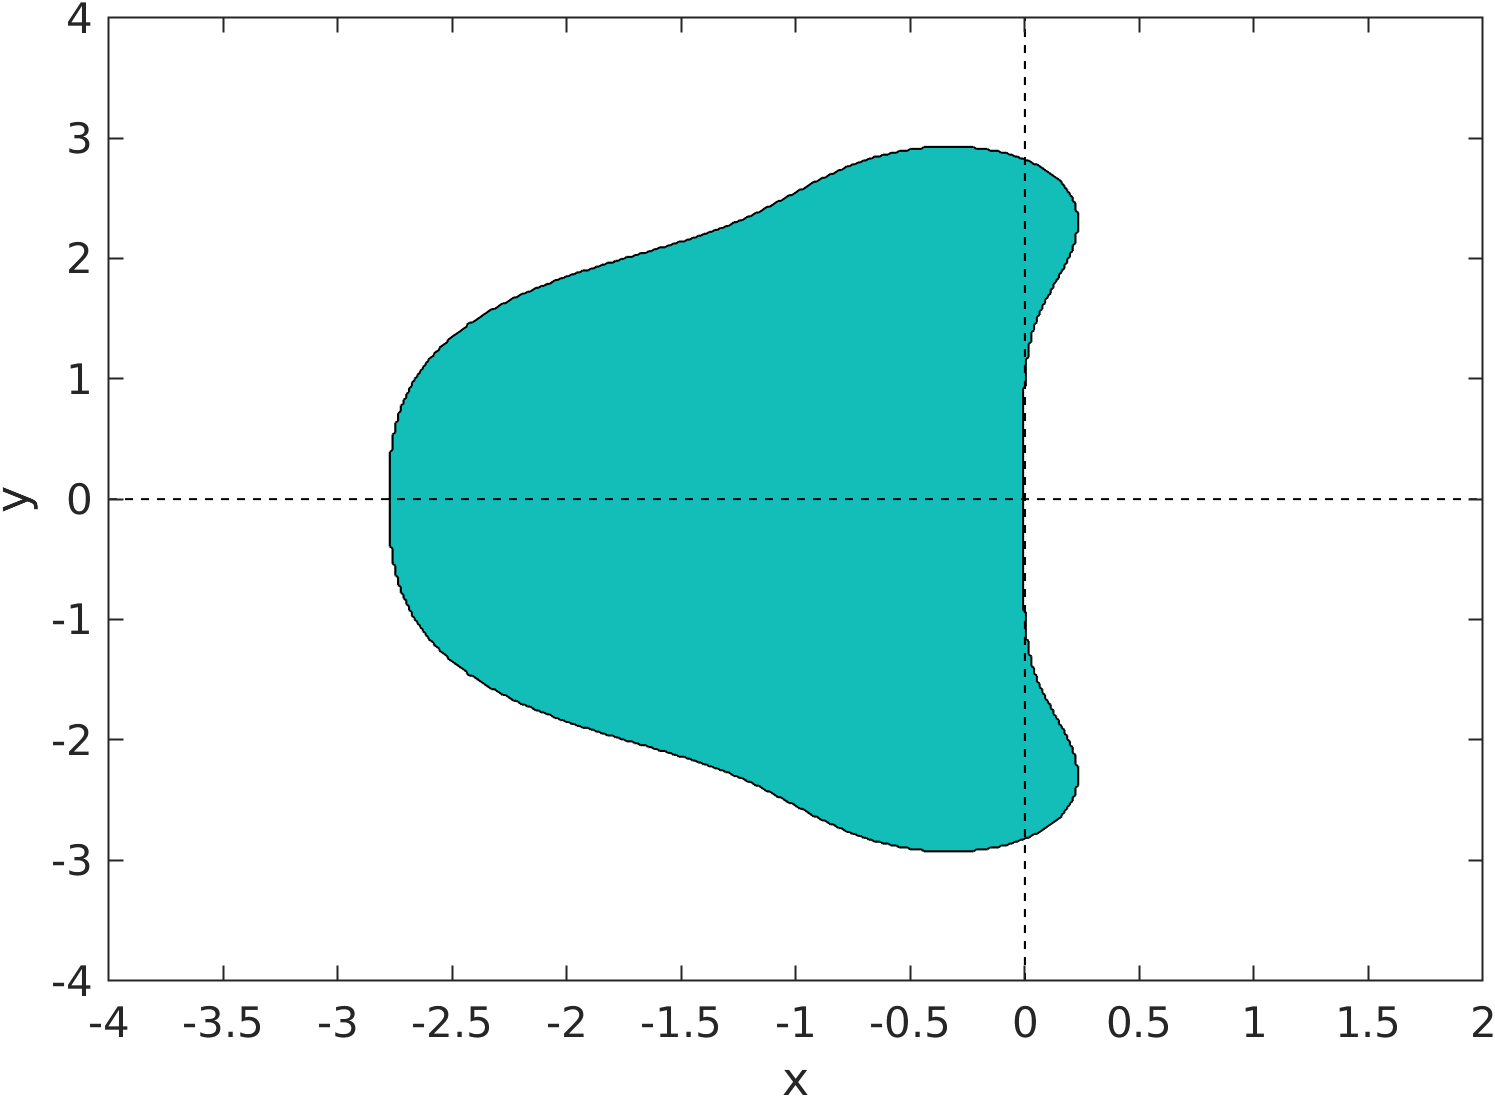
\includegraphics[height=0.35\textheight]{regione-RK-classico.png}
\caption{Regione di assoluta stabilità del metodo Runge-Kutta classico.}
\label{fig:regione-RK-classico}
\end{figure}

Per questo motivo, abbiamo scritto il Programma \ref{prog:plot-stability-region},
che disegna in modo approssimato la regione di assoluta stabilità del metodo
Runge-Kutta classico tramite un approccio di forza bruta basato su una griglia
regolare (la posizione e la dimensione della griglia sono state scelte a posteriori
in modo da ricoprire $\mathcal{D}$).
In ogni punto $q$ della griglia, il Programma \ref{prog:is-in-stability-region}
permette di stabilire se $q$ appartenga o meno a $\mathcal{D}$,
dopodiché la funzione \code{contourf} di MATLAB (basata sull'algoritmo
\emph{marching squares}) disegna sulla griglia un'approssimazione lineare a tratti
delle curve di livello della funzione caratteristica
dei punti $q$ interni a $\mathcal{D}$. La risoluzione dell'immagine risultante
(Figura \ref{fig:regione-RK-classico}) è pertanto la stessa della griglia,
che in questo esempio abbiamo scelto 500x500. Osserviamo che, se $\lambda \in \R^-$,
la restrizione sul passo $h$ affinché $q \in \mathcal{D}$ è circa $h \abs{\lambda} < 2.8$.

\section{Hamiltonian Boundary Value Methods}

Vediamo ora metodi numerici in grado di fornire discretizzazioni qualitativamente
corrette non solo nel caso dissipativo, ma anche nel caso conservativo.
Concentriamo l'attenzione su un particolare intervallo di tempo discreto
$[t_n,t_{n+1}]$, e cerchiamo un polinomio $u(t_n+ch)$ di grado $s$ che
approssimi la soluzione esatta $y(t_n+ch)$ per $c \in [0,1]$.
Dato che i polinomi di Legendre $P_j(c)$ shiftati e normalizzati
sull'intervallo $[0,1]$ formano un sistema ortonormale completo in $L^2([0,1])$,
sotto le dovute ipotesi di regolarità la derivata della soluzione $y'(t_n+ch)$
è uguale alla propria serie di Fourier rispetto alla base $\{P_j\}_{j \in \N}$:
\[
y'(t_n+ch) = \sum_{j=0}^{+\infty} \gamma_j P_j(c), \quad
\text{con } \gamma_j = \int_0^1 y'(t_n+ch) P_j(c) \dc
= \int_0^1 f(y(t_n+ch)) P_j(c) \dc.
\]
Da qui, l'idea degli \emph{Hamiltonian Boundary Value Methods} è quella di
cercare un polinomio $u(t_n+ch)$ che soddisfi una versione discreta e
finito-dimensionale dell'equazione precedente:
\begin{equation} \label{eq:discretizzazione-serie-di-fourier}
u'(t_n+ch) = \sum_{j=0}^{s-1} \hat{\gamma_j} P_j(c), \quad
\text{con } \hat{\gamma_j} = \sum_{\ell=1}^k b_\ell f(u(t_n + c_\ell h)) P_j(c_\ell)
\end{equation}
La serie di Fourier è stata dunque troncata dopo $s$ termini, mentre l'integrale
sull'intervallo $[0,1]$ è stato approssimato mediante formula di quadratura
su $k$ nodi $c_1,\dots,c_k$ con pesi $b_1,\dots,b_k$.
Sia $y_n$ l'approssimazione di $y(t_n)$ a ogni passo del metodo numerico.
Allora, la condizione $u(t_n) = y_n$ e le $s$ condizioni scalari sulla derivata
di $u(t_n+ch)$ determinano in modo univoco il polinomio $u \in \Pi_s$ cercato,
il cui valore in $t_{n+1}$ fornisce la nuova approssimazione $y_{n+1} \approx y(t_{n+1})$:
\begin{gather*}
\int_0^1 u'(t_n+ch) \dc
= \int_0^1 \, \sum_{j=0}^{s-1} \hat{\gamma_j} P_j(c) \dc
\qquad u(t_{n+1}) - u(t_n)
= h \int_0^1 \, \sum_{j=0}^{s-1} \hat{\gamma_j} P_j(c) \dc \\
y_{n+1}
= y_n + h \sum_{j=0}^{s-1} \hat{\gamma_j} \int_0^1 \! P_j(c) \dc
= y_n + h \hat{\gamma_0}
= y_n + h \sum_{\ell=1}^k b_\ell f(u(t_n+c_\ell h)).
\end{gather*}
Vista la somiglianza di questa equazione con la \eqref{eq:sistema-yn+1-runge-kutta}
(anche se qui, per semplicità, siamo nel caso omogeneo), chiamiamo $Y_i$
i valori $u(t_n + c_i h)$ al variare di $i = 1,\dots,k$ e integriamo nuovamente
la \eqref{eq:discretizzazione-serie-di-fourier}, stavolta da $0$ a $c_i$:
\begin{gather*}
\int_0^{c_i} u'(t_n+ch) \dc
= \int_0^{c_i} \, \sum_{j=0}^{s-1} \hat{\gamma_j} P_j(c) \dc
\qquad u(t_n + c_i h) - u(t_n)
= h \int_0^1 \, \sum_{j=0}^{s-1} \hat{\gamma_j} P_j(c) \dc \\
Y_i
= y_n + h \sum_{j=0}^{s-1} \hat{\gamma_j} \int_0^{c_i} \! P_j(c) \dc
= y_n + h \sum_{j=0}^{s-1}
	\left( \sum_{\ell=1}^k b_\ell f(Y_\ell) P_j(c_\ell) \right)
	\! \int_0^{c_i} \! P_j(c) \dc \\
= y_n + h \sum_{\ell=1}^k
	\left( \sum_{j=0}^{s-1} \int_0^{c_i} \! P_j(c) \dc \, P_j(c_\ell) b_\ell \right)
	f(Y_\ell)
\eqd y_n + h \sum_{\ell=1}^k a_{i\ell} f(Y_\ell)
\end{gather*}
Abbiamo pertanto ottenuto un metodo Runge-Kutta a $k$ stadi, detto
\emph{Hamiltonian Boundary Value Method $(k,s)$} e solitamente abbreviato in HBVM($k,s$).
Si può dimostrare che la matrice di Butcher $A$ è uguale a
$\mathcal{I}_s \mathcal{P}_s \Omega$, con
\begin{gather*}
\mathcal{I}_s = \begin{pmatrix}
\int_0^{c_1} \! P_{0}(c) \dc & \hdots & \int_0^{c_1} \! P_{s-1}(c) \dc \\ 
\vdots & & \vdots \\ 
\int_0^{c_k} \! P_{0}(c) \dc & \hdots & \int_0^{c_k} \! P_{s-1}(c) \dc
\end{pmatrix},
\quad \mathcal{P}_s = \begin{pmatrix}
P_0(c_1) & \hdots & P_{s-1}(c_1) \\
\vdots & & \vdots \\
P_0(c_k) & \hdots & P_{s-1}(c_k)
\end{pmatrix},
\quad \Omega = \begin{pmatrix}
b_1 & & \\
& \ddots & \\
& & b_k
\end{pmatrix}.
\end{gather*}
Oltre ai parametri $k$ e $s$, a definire un metodo HBVM è anche la scelta della
particolare formula di quadratura con cui vengono approssimati i coefficienti
di Fourier
\[
\gamma_j = \int_0^1 f(u(t_n+ch)) P_j(c) \dc.
\]
Una scelta molto buona, per certi versi ottima, è quella della formula di
quadratura di Gauss-Legendre, perché ha ordine massimo $2k$ tra
tutte le formule di quadratura di tipo interpolatorio su $k$ nodi.
Per questo, adotteremo tale scelta per tutto il resto del capitolo.
Dunque, $c_i$ sarà l'$i$-esima radice del polinomio di Legendre $P_k$,
e $b_i$ sarà l'integrale da 0 a 1 dell'$i$-esimo polinomio della base
di Lagrange definita sulle ascisse $c_1,\dots,c_k$. Sotto queste ipotesi,
si può dimostrare che i metodi HBVM($k,s$) hanno ordine $2s$ e sono
perfettamente A-stabili:

\begin{teor} \label{teorema-ordine-convergenza-HBVM}
Se $y_n = y(t_n)$ e $k \geq s$, allora l'approssimazione $y_{n+1}$ fornita
dal metodo HBVM($k,s$) soddisfa $y_{n+1}-y(t_{n+1}) = O(h^{2s+1})$.
In altre parole, il metodo HBVM($k,s$) ha errore di troncamento locale
dell'ordine di $h^{2s+1}$.
\end{teor}

\begin{teor}
Se $k \geq s$, la regione di assoluta stabilità del metodo HBVM($k,s$) è $\C^-$.
\end{teor}

\noindent Come anticipato, possiamo concludere che per i metodi Runge-Kutta
non vale un risultato analogo alla seconda barriera di Dahlquist
\ref{teor:seconda-barriera-dahlquist}.

\section{Problemi hamiltoniani}

Osserviamo che, da un punto di vista formale, i metodi HBVM($k,s$) sono metodi
Runge-Kutta a $k$ stadi, tuttavia il loro ordine di convergenza è funzione di $s$,
e questo non è sorprendente perché stiamo pur sempre approssimando $y(t)$
con un polinomio $u(t)$ di grado $s$, non $k$.
Ma, allora, perché non scegliere sempre $s=k$?
I motivi sono sostanzialmente due, e hanno a che fare con la soluzione
di problemi conservativi, di tipo hamiltoniano:

\begin{defi}
Si dice \emph{problema hamiltoniano} un problema della forma
\begin{equation} \label{eq:problema-hamiltoniano-qp}
\left\{
\begin{aligned}
q'(t)  &= \partial_p H (q(t),p(t)) \quad \text{per ogni $t \in [t_0,T]$}, \\
p'(t)  &= - \partial_q H (q(t),p(t)) \quad \text{per ogni $t \in [t_0,T]$}, \\
q(t_0) &= q_0 \in \R^m, \quad p(t_0) = p_0 \in \R^m,
\end{aligned}
\right.
\end{equation}
con $H(q,p) \colon \R^m \times \R^m \to \R^m$ funzione differenziabile
detta \emph{hamiltoniana}.
\end{defi}

\noindent Il caso del moto di una particella di massa $M$ in un campo
di forze conservative in $\R^m$ con potenziale $U$
\[
q''(t) = -\grad U(q) \in \R^m
\]
è un esempio di problema hamiltoniano con
\[
H(q,p) = \frac{1}{2M} \norm{p}^2 + U(q),
\]
infatti $q'(t) = p(t)/M$, $p'(t) = -\grad U(q(t))$.
Il problema \eqref{eq:problema-hamiltoniano-qp} può essere scritto in forma
più compatta nell'incognita $y(t) = (q(t),p(t))^T$ nel modo seguente:
\begin{equation*} \label{eq:problema-hamiltoniano-y}
\left\{
\begin{aligned}
y'(t)  &= J \grad H (y(t)) \quad \text{per ogni $t \in [t_0,T]$}, \\
y(t_0) &= y_0 = (q_0,p_0) \in \R^{2m},
\end{aligned}
\right.
\quad J = \begin{pmatrix}
0 & I_m \\ 
-I_m & 0
\end{pmatrix},
\quad \grad H(y) = \begin{pmatrix}
\partial_q H(y) \\ 
\partial_p H(y)
\end{pmatrix} 
\end{equation*}
Il valore dell'hamiltoniana $H(y)$ è un invariante lungo il moto di ogni sistema
hamiltoniano, infatti
\[
\frac{d}{dt} H(y(t)) = \grad H (y(t))^T J \grad H(y(t)) = 0,
\]
perché $J$ è una matrice antisimmetrica. Abbiamo dunque un'importante proprietà
qualitativa del moto che vorremmo preservare nel processo di discretizzazione
dell'equazione differenziale. In effetti, questa è la ragion d'essere
dei metodi HBVM e il primo dei due motivi per cui ha senso scegliere $k > s$:

\begin{teor}
Discretizzando un sistema hamiltoniano con un metodo HBVM($k,s$) con $k \geq s$
si ha che $H(y_{n+1}) - H(y_n) = O(h^{2k+1})$.
\end{teor}

\noindent Come corollario, si dimostra facilmente per mezzo della disuguaglianza
triangolare che
\[
\max_{0 \leq n \leq N} \Bigl\lbrace \abs{H(y_n)-H(y_0)} \Bigr\rbrace
= O(h^{2k}), \quad \text{con $N = (T-t_0)h^{-1}$.}
\]
Allora, è sufficiente scegliere $k$ tale che
$h^{2k} \approx \varepsilon = 1.1 \cdot 10^{-16}$ per avere
una conservazione \emph{pratica} dell'hamiltoniana,
cioè una conservazione non \emph{esatta}, ma entro i limiti della
precisione di macchina (meglio di così non si può fare, né c'è veramente
bisogno di farlo). Osserviamo che questa proprietà di conservazione dell'hamiltoniana
è indipendente dall'ordine $2s$ del metodo, anche se, a parità di
ordine di convergenza, i metodi conservativi hanno senz'altro un errore
più piccolo.

Il secondo motivo per cui ha senso scegliere $k > s$ è che, nonostante
il metodo HBVM($k,s$) sia da un punto di vista formale un metodo Runge-Kutta
a $k$ stadi, non è strettamente necessario risolvere il sistema non lineare
\[
F(Y) = Y - e \otimes y_n - h(A \otimes I_{2m}) f(Y)
\]
di dimensione $2mk$: il polinomio $u$ ha grado $s$ e quindi è inutile andare
a calcolare i suoi valori $Y_i = u(t_n + c_i h)$ in $k > s$ punti distinti.
Cambiamo allora punto di vista, e cerchiamo di ottenere un sistema chiuso
di equazioni per gli $s$ coefficienti di Fourier $\hat{\gamma_j} \in \R^{2m}$:
\begin{gather}
\hat{\gamma_j}
= \sum_{\ell=1}^k b_\ell f(u(t_n + c_\ell h)) P_j(c_\ell)
\qquad u(t_n + c_\ell h)
= y_n + h \sum_{j=0}^{s-1} \hat{\gamma_j} \int_0^{c_\ell} \! P_j(c) \dc \\
\label{eq:sistema-gamma-runge-kutta}
\hat{\gamma_j}
= \sum_{\ell=1}^k b_\ell \, f \left(
	y_n + h \sum_{i=0}^{s-1} \hat{\gamma_i} \int_0^{c_\ell} \! P_i(c) \dc
	\right) P_j(c_\ell)
\end{gather}
Le equazioni non lineari \eqref{eq:sistema-gamma-runge-kutta} al variare
di $j = 0,\dots,s-1$ formano un sistema di dimensione $2ms$,
la cui soluzione permette di avanzare nel tempo mediante la formula
$y_{n+1} = y_n + h \hat{\gamma_0}$. Ancora una volta, possiamo scegliere
se risolvere il sistema non lineare tramite il metodo di punto fisso,
il metodo di Newton, una variante di quest'ultimo o altro ancora.
In ogni caso, la complessità computazionale avrà una dipendenza molto
debole da $k$, il che significa che nella pratica possiamo sempre scegliere
$k$ in modo che il metodo preservi l'hamiltoniana.
Osserviamo che nel caso dei metodi HBVM le tolleranze per il criterio
di arresto misto sulle iterate vanno scelte dell'ordine di $h^{2k+1}$
anziché $h^{2s+1}$, altrimenti l'errore di troncamento sulla funzione
hamiltoniana dovuto all'algoritmo iterativo per la soluzione del
sistema non lineare prende il sopravvento sull'errore di troncamento
dovuto alla discretizzazione HBVM, e questo ci potrebbe impedire di avere
una conservazione pratica della funzione hamiltoniana.

\subsection*{Il problema di Keplero}

Vediamo ora un esempio di problema hamiltoniano: il
\emph{problema di Keplero}
\[
q'(t) = p(t)/m_2,
\quad p'(t) = -G \frac{m_1 m_2}{\norm{q(t)}^3} q(t),
\quad q(t), p(t) \in \R^2
\]
che descrive il moto in $\R^2$ di un corpo di massa $m_2$ attorno
a un corpo inamovibile posizionato nell'origine di massa $m_1 \gg m_2$
per effetto della forza di gravità ($G$ è la costante di gravitazione universale).
Questo sistema dinamico permette di modellare ad esempio il moto della Terra
intorno al Sole. La funzione hamiltoniana del problema di Keplero è
\[
H(q,p) = \frac{1}{2m_2} \norm{p}^2 - G \frac{m_1 m_2}{\norm{q}},
\]
con derivate parziali
\[
\partial_q H(q,p) = G \frac{m_1 m_2}{\norm{q}^3} q
\quad \text{e} \quad
\partial_p H(q,p) = p/m_2,
\]
e il suo valore $H(q,p)$ va interpretato come l'energia del sistema meccanico nel punto
$(q,p)$ del piano delle fasi; il fatto che $H$ sia una costante del moto
esprime quindi il principio di conservazione dell'energia per questo sistema
e il fatto che il moto sia vincolato alla varietà definita implicitamente
dalla curva di livello $H(q,p) = H(q_0,p_0)$.
Scegliendo valori matematicamente semplici per le varie costanti
($m_1 = 1$, $m_2=1$, $G = 1$), si può dimostrare che le condizioni iniziali
\[
y_0 = \begin{pmatrix}
q_0 \\ 
p_0
\end{pmatrix}, \quad
q_0 = \begin{pmatrix}
1-\varepsilon \\ 
0
\end{pmatrix}, \quad
p_0 = \begin{pmatrix}
0 \\ 
\sqrt{(1+\varepsilon)/(1-\varepsilon)}
\end{pmatrix}
\]
al variare di $\varepsilon$ in $[0,1)$ danno luogo a soluzioni $y(t)$ periodiche
di periodo $2\pi$ e che il grafico della curva $t \to q(t)$ è un'ellisse
di eccentricità $\varepsilon$. Oltre alla conservazione dell'energia,
abbiamo pertanto un'altra proprietà qualitativa importante delle soluzioni
che vorremmo preservare durante il processo di discretizzazione: il fatto che
il moto sia periodico e si svolga lungo una curva chiusa.

Come si comportano a riguardo i metodi numerici visti finora?
Nella Figura \ref{fig:confronto-traiettorie-keplero} abbiamo messo a confronto
le traiettorie fornite da quattro metodi di ordine 2 nel caso
\[
t_0 = 0, \quad
T = 20\pi, \quad
\varepsilon = 0.6, \quad
h = 3 \cdot 10^{-2}, \quad
G = 1, \quad
m_1 = 1, \quad
m_2 = 1.
\]
Il punto iniziale $y_0$ è stato marcato con una croce blu, mentre il punto
finale $y_N$ è stato marcato con un cerchio rosso. Dato che la soluzione esatta
ha periodo $2\pi$, in teoria $y_N$ dovrebbe coincidere con $y_0$,
o quanto meno trovarsi a una distanza dell'ordine di $h^2$.
Osserviamo invece che tutti i metodi hanno un punto finale piuttosto lontano
da $y_0$, con la sola eccezione del metodo HBVM conservativo in cui
effettivamente $\abs{y_N-y_0} \approx h^2$.
La BDF tende infatti a dissipare artificialmente l'energia del sistema,
provocando così una dilatazione del periodo del moto e un fenomeno di ritardo
del passaggio da $y_0$, mentre il metodo di Adams-Bashforth tende ad accrescere
artificialmente l'energia del sistema, provocando così una riduzione del periodo
del moto e un'anticipazione del passaggio da $y_0$ (fenomeno di \emph{overshooting}).
Il metodo dei trapezi si comporta un po' meglio degli altri due, perché
presenta una minore dispersione delle traiettorie (al pari di HBVM)
e perché evita una deriva dell'energia del sistema (ma a differenza di HBVM
la quantità $H(y_n)$ non è costante, perché oscilla tra -0.49 e -0.5).
Tuttavia, anche nel caso del metodo dei trapezi il risultato finale non
può essere considerato soddisfacente, perché il punto finale $y_N$
viene anticipato di molto rispetto a $y(t_N)$, e quindi già dopo 10 periodi si è persa
la qualità periodica del moto (o meglio, il fatto che il moto abbia periodo costante).

\begin{figure}[p]
\centering
\subcaptionbox{Metodo di Adams-Bashforth a due passi.} {
	\begin{tikzpicture}[trim axis left, trim axis right]
	\begin{axis}[
		width=0.55\textwidth,
		height=0.55\textwidth,
	]
	\addplot[black] table[x=y1, y=y2] {keplero-adams-bashforth.dat};
	\addplot[blue, only marks, mark=x, mark size=0.5em, line width=0.3em]
		coordinates{(0.4,0)};
	\addplot[red, only marks, mark=o, mark size=0.5em, line width=0.3em]
		coordinates{(-0.6009,1.2637)};
	\end{axis}
	\end{tikzpicture}
} \hfill
\subcaptionbox{Metodo dei trapezi (Adams-Moulton a un passo).} {
	\begin{tikzpicture}[trim axis left, trim axis right]
	\begin{axis}[
		width=0.55\textwidth,
		height=0.55\textwidth,
	]
	\addplot[black] table[x=y1, y=y2] {keplero-adams-moulton.dat};
	\addplot[blue, only marks, mark=x, mark size=0.5em, line width=0.3em]
		coordinates{(0.4,0)};
	\addplot[red, only marks, mark=o, mark size=0.5em, line width=0.3em]
		coordinates{(-0.9397,-0.84783)};
	\end{axis}
	\end{tikzpicture}
} \\[0.75em]
\subcaptionbox{BDF a due passi.} {
	\begin{tikzpicture}[trim axis left, trim axis right]
	\begin{axis}[
		width=0.55\textwidth,
		height=0.55\textwidth,
	]
	\addplot[black] table[x=y1, y=y2] {keplero-BDF.dat};
	\addplot[blue, only marks, mark=x, mark size=0.5em, line width=0.3em]
		coordinates{(0.4,0)};
	\addplot[red, only marks, mark=o, mark size=0.5em, line width=0.3em]
		coordinates{(-0.23124,-0.97329)};
	\end{axis}
	\end{tikzpicture}
} \hfill
\subcaptionbox{HBVM(5,1).} {
	\begin{tikzpicture}[trim axis left, trim axis right]
	\begin{axis}[
		width=0.55\textwidth,
		height=0.55\textwidth,
	]
	\addplot[black] table[x=y1, y=y2] {keplero-HBVM51.dat};
	\addplot[blue, only marks, mark=x, mark size=0.5em, line width=0.3em]
		coordinates{(0.4,0)};
	\addplot[red, only marks, mark=o, mark size=0.5em, line width=0.3em]
		coordinates{(0.4008,0.004986)};
	\end{axis}
	\end{tikzpicture}
}
\caption{Confronto tra metodi per il problema di Keplero con $\varepsilon = 0.6$.
La croce blu indica il punto iniziale di ogni traiettoria, il cerchio rosso il punto finale.}
\label{fig:confronto-traiettorie-keplero}
\end{figure}

A conclusione di questo paragrafo, e dell'intero elaborato, verifichiamo
numericamente le due proprietà per cui ha senso scegliere $k > s$ in un metodo
HBVM, e cioè che il massimo errore su $H$ nella soluzione di un problema
hamiltoniano tende a zero come $h^{2k}$ e che il metodo HBVM($k,s$)
possa essere implementato in modo tale da avere un costo computazionale
con dipendenza molto debole da $k$.

Nella Figura \ref{fig:errore-hamiltoniana-HBVM} abbiamo messo a confronto
il massimo errore sull'hamiltoniana prodotto da alcuni metodi HBVM($k,s$)
al variare di $k$ e $s$ nel caso del problema di Keplero con $t_0 = 0$,
$T = 20\pi$, $\varepsilon = 0.6$: possiamo osservare un ottimo accordo
con la teoria, entro i limiti della precisione di macchina.
Come avevamo già notato nell'analisi degli errori delle BDF
(Figura \ref{fig:lmf-BDF-convergenza}), l'epsilon di macchina non viene però raggiunto,
perché gli errori dovuti all'aritmetica finita sono una funzione crescente di $h^{-1}$:
in questo caso l'errore sull'hamiltoniana non scende sotto $10^{-14}$
(per fare meglio di così, bisognerebbe applicare a ogni passo uno
step correttivo all'hamiltoniana).

\begin{figure}[p]
\centering
\begin{tikzpicture}[trim axis left, trim axis right]
\begin{loglogaxis}[
	xlabel={$h$},
	ylabel={$\max \abs{H(y_n)-H(y_0)}$},
	width=0.9\textwidth,
	height=0.8\textheight,
	ymin=1e-20,
	legend style={anchor=south east,at={(0.975,0.025)}}
]
\addplot table {errH-HBVM11.dat};
\addplot table {errH-HBVM21.dat};
\addplot table {errH-HBVM31.dat};
\addplot table {errH-HBVM41.dat};
\addplot table {errH-HBVM22.dat};
\addplot table {errH-HBVM32.dat};
\addplot table {errH-HBVM42.dat};
\addplot[dashed, domain=1e-3:1e-1] expression {x^2};
\addplot[dashed, domain=1e-3:1e-1] expression {2*x^4};
\addplot[dashed, domain=1e-3:1e-1] expression {max(2.2e-16,4*x^6)};
\addplot[dashed, domain=1e-3:1e-1] expression {max(2.2e-16,4*x^8)};
\legend{$k=1,s=1,O(h^2)$\\$k=2,s=1,O(h^4)$\\$k=3,s=1,O(h^6)$\\$k=4,s=1,O(h^8)$\\
                          $k=2,s=2,O(h^4)$\\$k=3,s=2,O(h^6)$\\$k=4,s=2,O(h^8)$\\}
\end{loglogaxis}
\end{tikzpicture}
\caption{Verifica dell'ordine dell'errore globale sull'hamiltoniana per metodi HBVM($k,s$).}
\label{fig:errore-hamiltoniana-HBVM}
\end{figure}

Per quanto riguarda la seconda verifica sperimentale, abbiamo messo a
confronto due implementazioni del metodo HBVM($k,s$): la prima tratta
il metodo come un qualunque metodo Runge-Kutta a $k$ stadi implicito
e consiste nell'esecuzione del Programma \ref{prog:runge-kutta} con $(b,c)$ dati dalla
formula di quadratura di Gauss-Legendre e $A = \mathcal{I}_s \mathcal{P}_s \Omega$,
mentre la seconda è basata sulla risoluzione del sistema
\eqref{eq:sistema-gamma-runge-kutta} (ulteriormente semplificato)
e consiste nell'esecuzione della function \code{hbvm} che abbiamo scaricato dalla pagina
\[
\text{\url{http://web.math.unifi.it/users/brugnano/LIMbook/software.html}}
\]
Dei programmi pubblicati su tale pagina, abbiamo anche fatto uso
della function \code{RKform} per generare la terna $(A,b,c)$
e della function \code{kepler} per fornire $H(y)$ e $\grad H(y)$ del problema
di Keplero a \code{hbvm}. Lo step correttivo dell'hamiltoniana (sottofunzione
\code{correggiH}) è stato disattivato per generare i risultati nella
Figura \ref{fig:errore-hamiltoniana-HBVM}.

Nella Figura \ref{fig:confronto-tempi-esecuzione-HBVM} abbiamo riportato il tempo
di esecuzione richiesto dalle due implementazioni del metodo HBVM($k,s$)
per la simulazione del problema di Keplero con parametri
\[
t_0 = 0, \quad
T = 20\pi, \quad
\varepsilon = 0.6, \quad
h = 10^{-2}, \quad
G = 1, \quad
m_1 = 1, \quad
m_2 = 1.
\]
al variare di $k$ e $s$. Come preannunciato, possiamo osservare che
il costo computazionale dell'implementazione ingenua è direttamente proporzionale
a $k$, mentre il tempo di esecuzione richiesto dalla function
\code{hbvm} è sensibile unicamente al parametro $s$, peraltro in modo
molto debole: a parità di ordine di convergenza,
i metodi conservativi con $k > s$ non hanno quindi un costo
computazionale maggiore, a patto che siano implementati in modo opportuno.

\begin{figure}[tbp]
\centering
\begin{tikzpicture}[trim axis left, trim axis right]
\begin{axis}[
	xlabel={$k$},
	ylabel={Tempo di esecuzione (secondi)},
	width=0.9\textwidth,
	height=0.5\textheight,
	legend style={anchor=north west,at={(0.025,0.975)}}
]
\addplot[red,mark=*]          table {benchmark-naive-HBVMk1.dat};
\addplot[red,mark=square*]    table {benchmark-naive-HBVMk2.dat};
\addplot[red,mark=triangle*]  table {benchmark-naive-HBVMk3.dat};
\addplot[red,mark=diamond*]   table {benchmark-naive-HBVMk4.dat};
\addplot[blue,mark=*]         table {benchmark-optimized-HBVMk1.dat};
\addplot[blue,mark=square*]   table {benchmark-optimized-HBVMk2.dat};
\addplot[blue,mark=triangle*] table {benchmark-optimized-HBVMk3.dat};
\addplot[blue,mark=diamond*]  table {benchmark-optimized-HBVMk4.dat};
\legend{$s=1$,$s=2$,$s=3$,$s=4$,$s=1$,$s=2$,$s=3$,$s=4$}
\end{axis}
\end{tikzpicture}
\caption{Confronto tra i tempi di esecuzione di due implementazioni del
metodo HBVM($k,s$).\\ Le curve in rosso si riferiscono al Programma
\ref{prog:runge-kutta}, mentre le curve in blu si riferiscono alla
function \code{hbvm}.}
\label{fig:confronto-tempi-esecuzione-HBVM}
\end{figure}


















